\documentclass{beamer}

% presentation themeing
\usetheme{Singapore}
\beamertemplatenavigationsymbolsempty
\setbeamertemplate{bibliography item}{\insertbiblabel}

% output configuration
\usepackage{pgfpages}
%\setbeameroption{show notes on second screen=left}
\hypersetup{pdfpagemode=FullScreen}

% type setting packages
\usepackage{algorithmic}
\usepackage{amsmath}
\usepackage{siunitx}
\usepackage{etoolbox}

%math typeseting
\newcommand{\mat}[1]{\mathbf{#1}}

% plotting setup
\usepackage{pgfplots}
	\pgfplotsset{compat=1.16}
\usepackage{pgfplotstable}

\pgfplotstableset{col sep=semicolon}

\pgfplotstableread{figures/4.Results/Vec.csv}\vectable
\pgfplotstableread{figures/4.Results/Ind.csv}\indtable
\pgfplotstableread{figures/4.Results/Val.csv}\valtable

% title slide
\title{\input{title.txt}}
\author{\textbf{Neil Lindquist}\\
All-College Thesis Defense}
\date{April 16th, 2019}

\begin{document}
\begin{frame}
	\titlepage
\end{frame}

% Motivation
\begin{frame}
	\frametitle{Goal}
	\begin{itemize}
		\item Sparse linear systems used by many scientific computations
		\item Problems can be large, with over a million variables
		\item Arithmetic is faster than fetching data from memory
		%TODO mention cache
	\end{itemize}
\end{frame}

% Data access patterns/compression limitations
\begin{frame}[fragile]
	\frametitle{Solver Description}
	\begin{itemize}
		\item Preconditioned Conjugate Gradient was used for tests
		\begin{itemize}
			\item Preconditioned with a 3 level multigrid
			\item Symmetric Gauss-Seidel step smoother
		\end{itemize}
		\item Matrix store in CSR format
		\begin{itemize}
			\item Stores the column index and value for each nonzero entry
		\end{itemize}
		3 compressible data structures
		\begin{itemize}
			\item Vector Values
			\item Matrix Indices
			\item Matrix Values
		\end{itemize}
	\end{itemize}
\end{frame}

%TODO consider describing test matrix

\begin{frame}
	\frametitle{Main Data Access Pattern}
	\begin{algorithmic}
		\FOR{row in rows}
			\FOR{nonzero entry in row}
				\STATE LOAD entry's value
				\STATE LOAD entry's column index
				\STATE LOAD vector value for column index
			\ENDFOR
			\STATE WRITE vector value for row
		\ENDFOR
	\end{algorithmic}
	
	\begin{itemize}
		\item need random vector reads
		\item need vector writes
		\item need both forward and backward iteration of matrix rows
	\end{itemize}
\end{frame}

% Model results

\begin{frame}
	\frametitle{Analytical Performance Model}
	\begin{itemize}
		\item System of equations that assumes no processor-level parallelism
		\item Solving for what conditions outperform the baseline gives:
	\end{itemize}
	\begin{align*}
%		\mathrm{vectEncode} <& 878.513 \\
		\mathrm{totalDecode} <& 32.5375 - 0.037037\cdot\mathrm{vectEncode} \\
		\mathrm{matBytes} <& 12.9664 - 0.398506\cdot\mathrm{totalDecode} \\
							&- 0.0147595\cdot\mathrm{vectEncode}\\
		\mathrm{vectBytes} <& 7.9998 + 8.27835\cdot(12 - \mathrm{matBytes}) \\
							&- 3.29897\cdot\mathrm{totalDecode}- 0.122184\cdot\mathrm{vectEncode}\\
	\end{align*}
\end{frame}

\begin{frame}
	\frametitle{Simulation Performance Model}
	\begin{itemize}
		\item Some processor level parallelism
		\item Conditions for outperforming the baseline:
	\end{itemize}
	
	%TODO consider switching to a graph
	\begin{tabular}{r|S|S|c}
      & {Matrix Index}  & {Matrix Value} & {Vector}\\
	{Bytes} & {Decode}        & {Decode}       & Encode and Decode \\
	\hline
	1 & 66 & 41 & \(4.75\geq 1.75\cdot\mathrm{decode}+\mathrm{encode}\)\\
	2 & 51 & 14 &\(4.75\geq 1.75\cdot\mathrm{decode}+\mathrm{encode}\)\\
	3 & 66 & 40 &\(2\geq 2\cdot\mathrm{decode}+\mathrm{encode}\)\\
	4 & 0 & 0 &\(0=\mathrm{decode}=\mathrm{encode}\) \\
	5 & {-} & 37 & \(4.75\geq 1.75\cdot\mathrm{decode}+\mathrm{encode}\)\\
	6 & {-} & 9 & Not Possible\\
	7 & {-} & 35 & \(0=\mathrm{decode}=\mathrm{encode}\)\\
	8 & {-} & 0 & \(0=\mathrm{decode}=\mathrm{encode}\)
\end{tabular}
\end{frame}

% Timing results
\begin{frame}
	\frametitle{Vector Compression}
	\raggedleft
	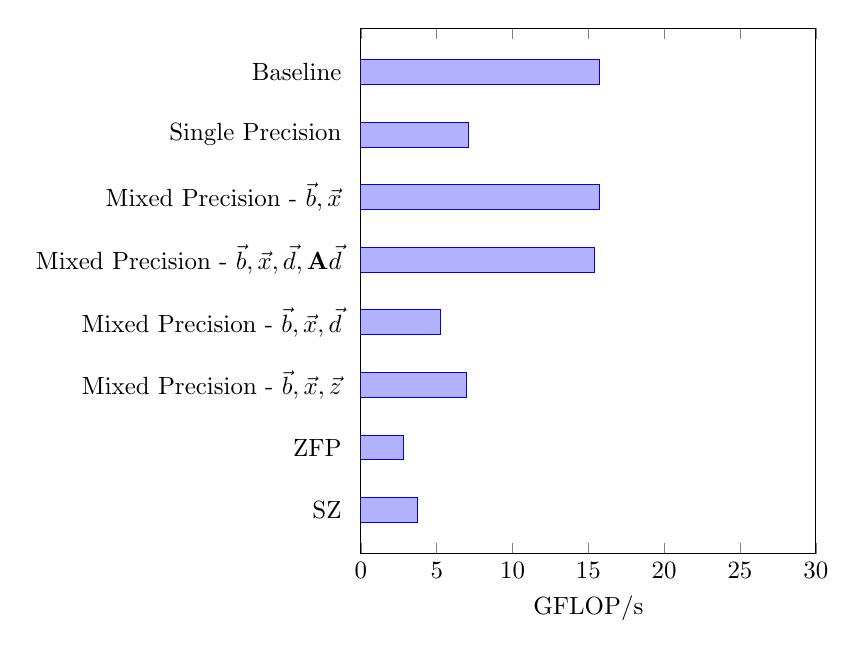
\begin{tikzpicture}[scale=.9]
		\begin{axis}[xbar,
					xlabel={GFLOP/s},
					xmin=0,
					xmax=30,
					width=8cm,
					height=9cm,
					ytick style={draw=none},
					symbolic y coords={{SZ},{ZFP},{Mixed Precision - b,x,z},{Mixed Precision - b,x,d},{Mixed Precision - b,x,Ad},{Mixed Precision - b,x},{Single Precision},{Baseline}},
					ytick={{SZ},{ZFP},{Mixed Precision - b,x,z},{Mixed Precision - b,x,d},{Mixed Precision - b,x,Ad},{Mixed Precision - b,x},{Single Precision},{Baseline}},
					yticklabels={{SZ},{ZFP},{Mixed Precision - \(\vec{b}, \vec{x}, \vec{z}\)},{Mixed Precision - \(\vec{b}, \vec{x}, \vec{d}\)},{Mixed Precision - \(\vec{b}, \vec{x}, \vec{d}, \mat{A}\vec{d}\)},{Mixed Precision - \(\vec{b}, \vec{x}\)},{Single Precision},{Baseline}} ]
			\addplot coordinates{
				(15.7394,Baseline)
				(7.10126,Single Precision)
				(15.7503,{Mixed Precision - b,x})
				(15.4048,{Mixed Precision - b,x,Ad})
				(5.25084,{Mixed Precision - b,x,d})
				(6.98823,{Mixed Precision - b,x,z})
				(2.80692,ZFP) %3d 14 bit
				(3.69907,SZ) %24 vals/block
			};
		\end{axis}
	\end{tikzpicture}
\end{frame}

\begin{frame}
	\frametitle{Matrix Value Compression}
	\raggedleft
	\begin{tikzpicture}[scale=.9]
		\begin{axis}[xbar,
					xlabel={GFLOP/s},
					xmin=0,
					xmax=30,
					width=8cm,
					height=9cm,
					ytick=data,
					ytick style={draw=none},
					yticklabels from table={\valtable}{graphname},
					y dir=reverse]
			\addplot table[x=gflops,y expr=\coordindex]{\valtable};
		\end{axis}
	\end{tikzpicture}
\end{frame}

\begin{frame}
	\frametitle{Matrix Index Compression}
	\raggedleft
	\begin{tikzpicture}[scale=.9]
		\begin{axis}[xbar,
					xlabel={GFLOP/s},
					xmin=0,
					xmax=30,
					width=8cm,
					height=9cm,
					ytick=data,
					ytick style={draw=none},
					yticklabels from table={\indtable}{graphname},
					y dir=reverse]
			\addplot table[x=gflops,y expr=\coordindex]{\indtable};
		\end{axis}
	\end{tikzpicture}
\end{frame}

\begin{frame}
	\frametitle{Matrix Value and Index Compression}
	\raggedleft
	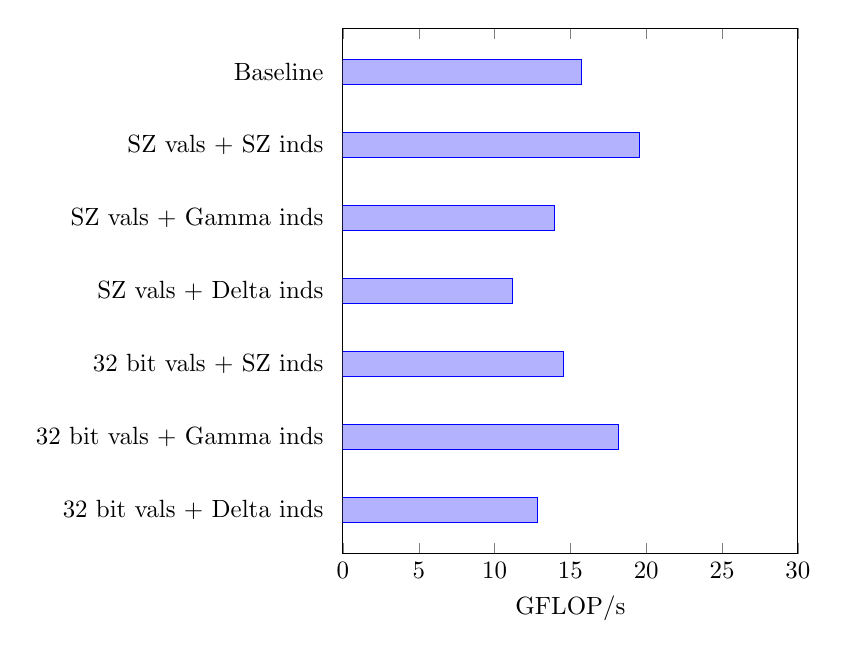
\begin{tikzpicture}[scale=.9]
		%TODO consider making this a grouped bar graph
		\begin{axis}[xbar,
					xlabel={GFLOP/s},
					xmin=0,
					xmax=30,
					width=8cm,
					height=9cm,
					y dir=reverse,
					ytick style={draw=none},
					symbolic y coords={{baseline},{sz-sz},{sz-gamma},{sz-delta},{32-sz},{32-gamma},{32-delta}},
					ytick            ={{baseline},{sz-sz},{sz-gamma},{sz-delta},{32-sz},{32-gamma},{32-delta}},
					yticklabels={{Baseline},{SZ vals + SZ inds},{SZ vals + Gamma inds},{SZ vals + Delta inds},{32 bit vals + SZ inds},{32 bit vals + Gamma inds},{32 bit vals + Delta inds}} ]
			\addplot coordinates{
				(15.7394,{baseline})
				(19.5759,{sz-sz})
				(13.9794,{sz-gamma})
				(11.1961,{sz-delta})
				(14.5156,{32-sz})
				(18.1835,{32-gamma})
				(12.8181,{32-delta})
			};
		\end{axis}
	\end{tikzpicture}
\end{frame}

\begin{frame}
	\frametitle{Vector and Matrix Compression}
	\raggedleft
	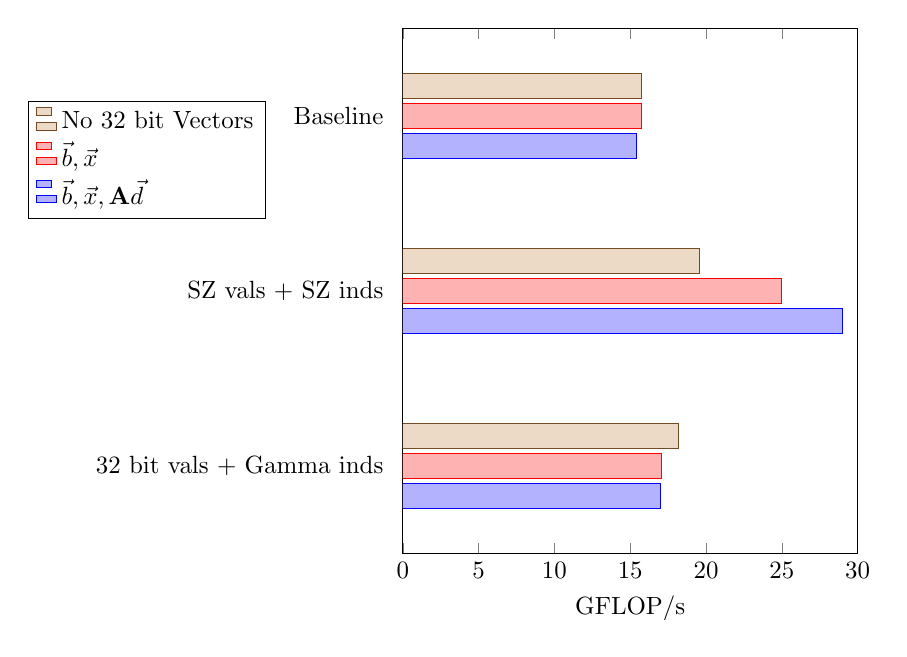
\begin{tikzpicture}[scale=.9]
		\begin{axis}[xbar,
					xlabel={GFLOP/s},
					xmin=0,
					xmax=30,
					width=8cm,
					height=9cm,
					y dir=reverse,
					ytick style={draw=none},
					symbolic y coords={Baseline,SZ,Gamma},
					ytick            ={Baseline,SZ,Gamma},
					yticklabels={{Baseline},{SZ vals + SZ inds},{32 bit vals + Gamma inds}},
					enlarge y limits=0.25,
					legend entries={{\(\vec{b},\vec{x},\mat{A}\vec{d}\)},{\(\vec{b},\vec{x}\)},{No 32 bit Vectors}},
					reverse legend=true,
					legend style={
						anchor=east,
						at={(axis description cs:-.3,.75)}
					},
					legend cell align=left,
					]
			\addplot coordinates{ %b,x,Ad single
				(15.4048,Baseline)
				(28.9699,SZ)
				(17.02944,Gamma)
			};
			\addplot coordinates{ %b,x single
				(15.7503,Baseline)
				(24.9875,SZ)
				(17.0684,Gamma)
			};
			\addplot coordinates{ %no single
				(15.7394,Baseline)
				(19.5759,SZ)
				(18.1835,Gamma)
			};
		\end{axis}
	\end{tikzpicture}
\end{frame}

% Select Compression methods
\begin{frame}
	\frametitle{Successful Compression Methods}
	\begin{itemize}
		\item Mixed Floating Point Precision
		\item SZ Compression
		\item Elias Gamma Coding
	\end{itemize}
\end{frame}

\begin{frame}
	\frametitle{Mixed Floating Point Precision}
	\begin{itemize}
		\item Single Precision takes half the storage space
		\item But drops from 15-17 significant digits to 6-9 digits
		\item Certain vectors can be lower precision without slowing convergence
	\end{itemize}
	%TODO this needs work
\end{frame}

\begin{frame}
	\frametitle{Squeeze ``SZ'' Compression}
	\begin{itemize}
		\item Stores a key for the predictor function with the best accuracy
		\item If can't be predicted within a minimum accuracy, sorted explicitly in a second list
		\item Available prediction functions are chosen based on the type of data
	\end{itemize}
\end{frame}
%TODO consider adding an example

\begin{frame}
	\frametitle{Elias Gamma Coding}
	\begin{itemize}
		\item Positive integers
		\item Stores number of bits needed then the data
		\item Very effective for small integers
		\begin{itemize}
			\item ``1'' takes 1 bit
		\end{itemize}
		\item Elias Delta Coding is similar, but Gamma codes the length 
	\end{itemize}
\end{frame}

% Conclusion
\begin{frame}
	\frametitle{Conclusion}
	\begin{itemize}
		\item Iterative linear solvers are memory access bound
		\item Compressing key data structures provided an 84\% increase in performance
	\end{itemize}
\end{frame}

\end{document}
